\chapter{Prediction of Delayed Wound Healing}
\section{Introduction}
\subsection{Chronic wounds}
Chronic wounds are those that fail to heal in a timely manner
\cite{Lazarus1994}, and affect an estimated 6.5 million people in the
United States (2\% of the population) \cite{Fife2012}.  Chronic wounds
are at increased risk of complications, such as amputation and
infection, which can have a severe negative impact on patient
well-being.  The cost of treating these wounds is high – up to \$50
billion annually \cite{Driver2010,Hess1996,Kuhn1992} – and the
incidence of chronic wounds is expected to increase due to an aging
population and rising risk factors such as diabetes and obesity
\cite{Sen2009}. Given accurate prognostic information, it may be
possible to triage patients for additional care such as additional
monitoring and at-home care, hyperbaric oxygen therapy (HBOT), and
negative pressure wound therapy (NPWT)
\cite{Andros2006,Clemens2008,Melling2006,Stojadinovic2008,Wu2008,Armstrong2008,Bozzuto2000}.
Thus an accurate prediction has the potential to change the course of
clinical treatment.

Previous work has attempted to identify factors of prognostic value in
predicting delayed wound healing, but most of these studies were
restricted to specific wound types such as venous leg ulcers
\cite{Margolis2003,Margolis2004,Cardinal2008,Ubbink2013,Kantor1998,Wicke2009}.
They used patient cohorts of modest size and drawn from single sites
or enrolled in clinical trials, limiting the generalizability of these
results to the diversity of patients and wound types seen in clinical
practice \cite{Carter2009}.  Furthermore, these models have not yet
been validated in independent datasets with respect to either
discriminatory power or calibration.

Among the best work to date is that of Margolis et
al. \cite{Margolis2003,Margolis2004} who developed prognostic models
for venous leg ulcers and diabetic neuropathic foot ulcers using data
from tens of thousands of patients across geographically diverse
outpatient wound care centers, and carefully validated the models,
achieving excellent calibration but only modest discriminative power
(AUCs ranging from 0.63 to 0.71).  These results led to the study by
Kurd et al. \cite{Kurd2009}, a clustered multicenter trial
demonstrating that providing prognostic information from these models
to clinicians improved healing rates even without specific guidance
about treatment options.

In this work, we report the development and validation of a novel
prognostic model that uses data routinely collected over the first
week of care at outpatient wound centers.  Our model achieves an AUC
of \textbf{CHANGE ME} 0.863 (95\% confidence interval 0.857-0.869) on
held out data and provides well-calibrated probabilities for delayed
wound healing.  Our model is constructed and validated on a dataset
comprising tens of thousands of patients with over a hundred thousand
wounds from geographically diverse wound care centers.  All wound
types are considered in this work, and thus the model is applicable to
the full diversity of wounds seen in clinical practice.

\subsection{Impact of Non-stationarity on Predictive Modeling}
The rapid adoption of electronic health records (EHRs) is a key
enabler of the learning healthcare system
\cite{Friedman2010,Weng2012,Shah2012,Bates2014,Embi2013}.  The most
immediate effect of EHR adoption is simply to vastly increase the
amount of data available for tasks such as predictive modeling of
clinical outcomes.  This increase in data enables developers of such
models to employ increasingly sophisticated models to improve
performance while still controlling for overfitting.  For example,
recent work has applied tensor factorization to discover latent
disease subtypes \cite{Ho2014}.  Such models are a far cry from the
logistic regression models that have long been a mainstay of clinical
research, and have the potential to transform clinical care.  However,
the nature of EHR derived data raises several practical issues in the
development of such models \cite{Hersh2013,Hripcsak2011,Paxton2013}.
Failure to take these issues into account in the development and
deployment of these models could lead to high profile failures that
could ultimately delay the learning healthcare system
\cite{Cook2011,Boland2013}.

EHR records typically have repeated observations of a constantly
evolving set of patients.  Furthermore, we note that the health care
system in the United States is currently, and for the foreseeable
future, in a state of flux, with new systems being adopted and
clinical practice evolving at a rapid pace as incentives change.
Indeed, we note that this situation is in fact an explicit goal of the
learning health care system.  We explore what such changes imply for
predictive modeling using EHR data.

The wound healing dataset we use to develop a predictive model
consists of wound and patient data collected over the course of care
at outpatient would care centers operated by Healogics Inc between
2009 and 2013.  In this setting, patients are seen on a weekly basis
to monitor the progress of wound healing and adjust care as
appropriate.  Quantitative and categorical descriptions of wounds are
entered into an EHR during each such assessment.  The objective of the
model is to predict whether or not a given wound will be an outlier
with respect to how long it takes to fully heal, given only
information collected during the first and second wound assessments.
The threshold for delayed wound healing was set to fifteen weeks based
on the observations of clinical experts at Healogics.

This dataset has several characteristics that we believe make it
especially illuminating with respect to developing and potentially
deploying predictive models in practice.  First, the dataset consists
of longitudinal observations of multiple wounds from many patients,
with no restrictions on the patient population or wound types.
Second, the data was collected from 68 geographically distributed
wound care centers.  Finally, Healogics expanded its operations by
both opening new wound care centers and taking over the operations of
other specialized wound care systems during the study period.
Healogics was also increasing adoption of its EHR, and it was apparent
from preliminary examination of the data that there were significant
changes in EHR use over the study period.  For instance, prior to 2013
there were many instances of wounds whose type was coded as ‘Diabetic
Wound, Lower Extremity’.  From 2013 onwards, this wound type almost
entirely disappeared, and was superseded by more specific categories
such as ‘Neuropathic diabetic wound’ and ‘Neuro-ischemic diabetic
wound’.  More generally, the prevalence of delayed wound healing was
lower in 2013 (i.e., the most recent data available for this study)
than previously (10.4\% versus 13.2\% respectively).  Thus, in this
dataset, there was significant non-stationarity, i.e., the process
generating the data changed over time.  This issue has long been known
to bedevil predictive models in other domains but receives relatively
little attention in the biomedical informatics literature
\cite{Bickel2009,Hoens2012,Moreno2011}.

We present experiments evaluating the impact of non-stationarity on
discriminative power (how well models distinguish between cases and
non-cases) and on model calibration (how closely the posterior
probabilities of delayed wound healing output by models match observed
frequencies of delayed wound healing).  We approximate different
degrees of stability of the data generating process by changing the
way that the data is split into training and test sets. We then
examine how such change impacts model selection.  To that end, we
consider the use of increasingly sophisticated models, starting from
regularized logistic regression, progressing through non-linear models
capable of automatically modeling interactions between predictors, and
ending with ensemble methods that combine the predictions of many base
models.  Finally, we examine the impact of non-stationarity on
engineered, domain specific features.

We demonstrate that in a setting that approximates a stationary data
distribution, ensemble methods such as stacking can provide
significant boosts to predictive power.  However, this performance
gain disappears when the data distribution is non-stationary.  In both
cases, however, there is consistent benefit from using engineered,
domain specific features.  We find that using non-linear models that
capture feature interactions automatically is useful in this dataset
but that the benefit from such models is reduced under
non-stationarity.  Our findings emphasize the importance of matching
the model development process with the intended use of the model. If
the model is intended for use on future patients, it is critical to
take non-stationarity into account to obtain a reliable estimate of
model performance.

\section{Materials and Methods}
Our goals are two-fold.  First, we aim to develop an accurate,
well-calibrated model for predicting delayed wound healing.  We also
aim to investigate the impact of non-stationarity on such models.  The
outcome we are trying to predict is whether or not a given wound will
take longer than 15 weeks to heal using information routinely
collected during the first week of care. We approach this by fitting a
series of increasingly complex models—with and without domain specific
features—to different training and test splits of the data.  We
observed that the dataset exhibits substantial non-stationarity.  We
can, however, control the degree of non-stationarity seen by the
models by changing the way we split the data.  We evaluate the models
for discriminative power and calibration under these different
conditions.  In the remainder of this section, we provide details
about the dataset, feature construction, model development and
evaluation.

\subsection{Dataset}
The dataset is comprised of 1,182,751 time-stamped wound assessments
performed at 68 Healogics outpatient wound care centers distributed
over 26 states from 2009 through 2013 (Figure 5.1).  These wound
assessments represented 180,716 unique wounds.  Each wound assessment
consists of both quantitative information regarding a specific wound,
such as length, width, depth and area, in addition to categorical
descriptors such as wound type, anatomical location, presence/absence
of erythema and ICD9 codes associated with the assessment.  Each
assessment is also associated with unique wound and patient keys,
allowing us to associate each wound with basic demographic information
such as age, gender, and insurance status along with its
outcome. Wound assessments were performed approximately weekly, and
the dataset spans 2009 through 2013.  There were 40 wound types (e.g.,
Pressure Ulcer, Venous Ulcer) and 37 anatomic locations.  The mean
duration of care was 52.2 days.  Overall, 11.6\% of wounds exhibited
delayed wound healing, defined as 15 or more weeks to closure. A total
of 59,958 patients are represented.  Figure 5.2 shows basic statistics
about the dataset.

\begin{figure}
  \begin{center}
    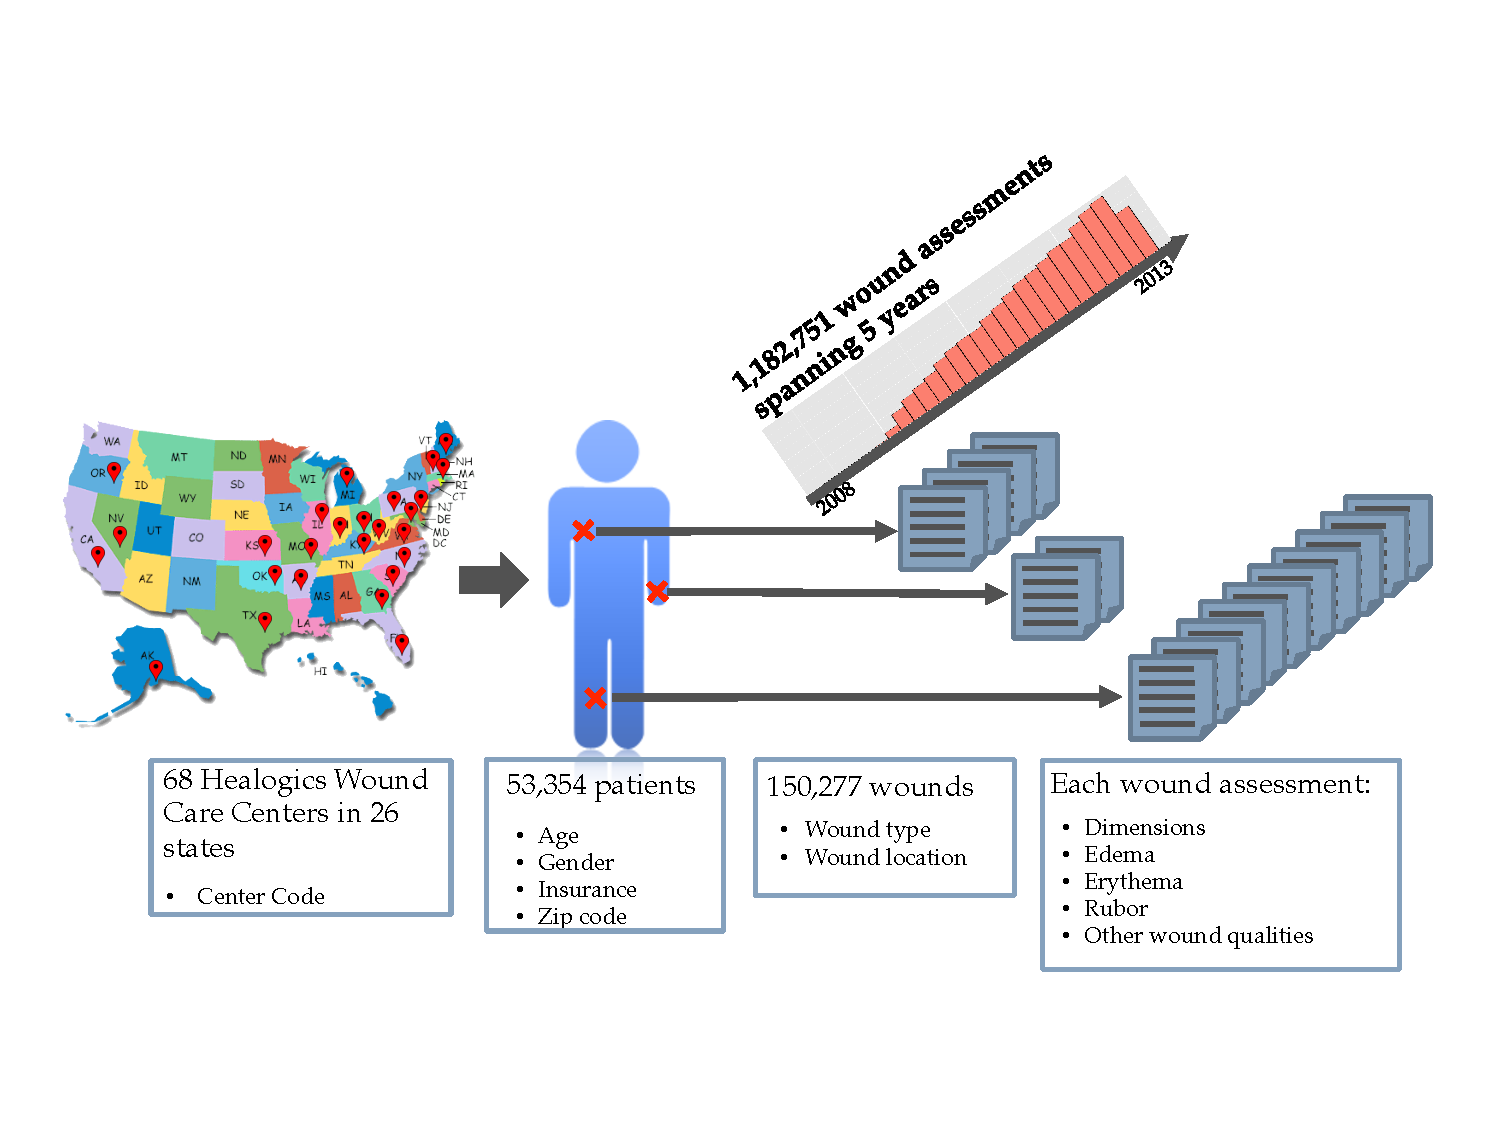
\includegraphics[width=0.9\linewidth]{ch5-figures/dataset_overview.pdf}
  \end{center}
  \caption[Wound healing dataset characteristics]{Dataset
    characteristics. The dataset is drawn from 68 Healogics wound care
    centers in 26 states over a period spanning 2009 through 2013 and
    comprises 181,716 wounds from 59,958 patients. Patient and wound
    information is recorded in an EHR at each weekly wound
    assessment. There were 40 distinct wound types spanning 37
    anatomical locations. We use the information recorded in the first
    two assessments to predict delayed wound healing.}
  \label{fig:short}
\end{figure}

\begin{figure}
  \begin{center}
    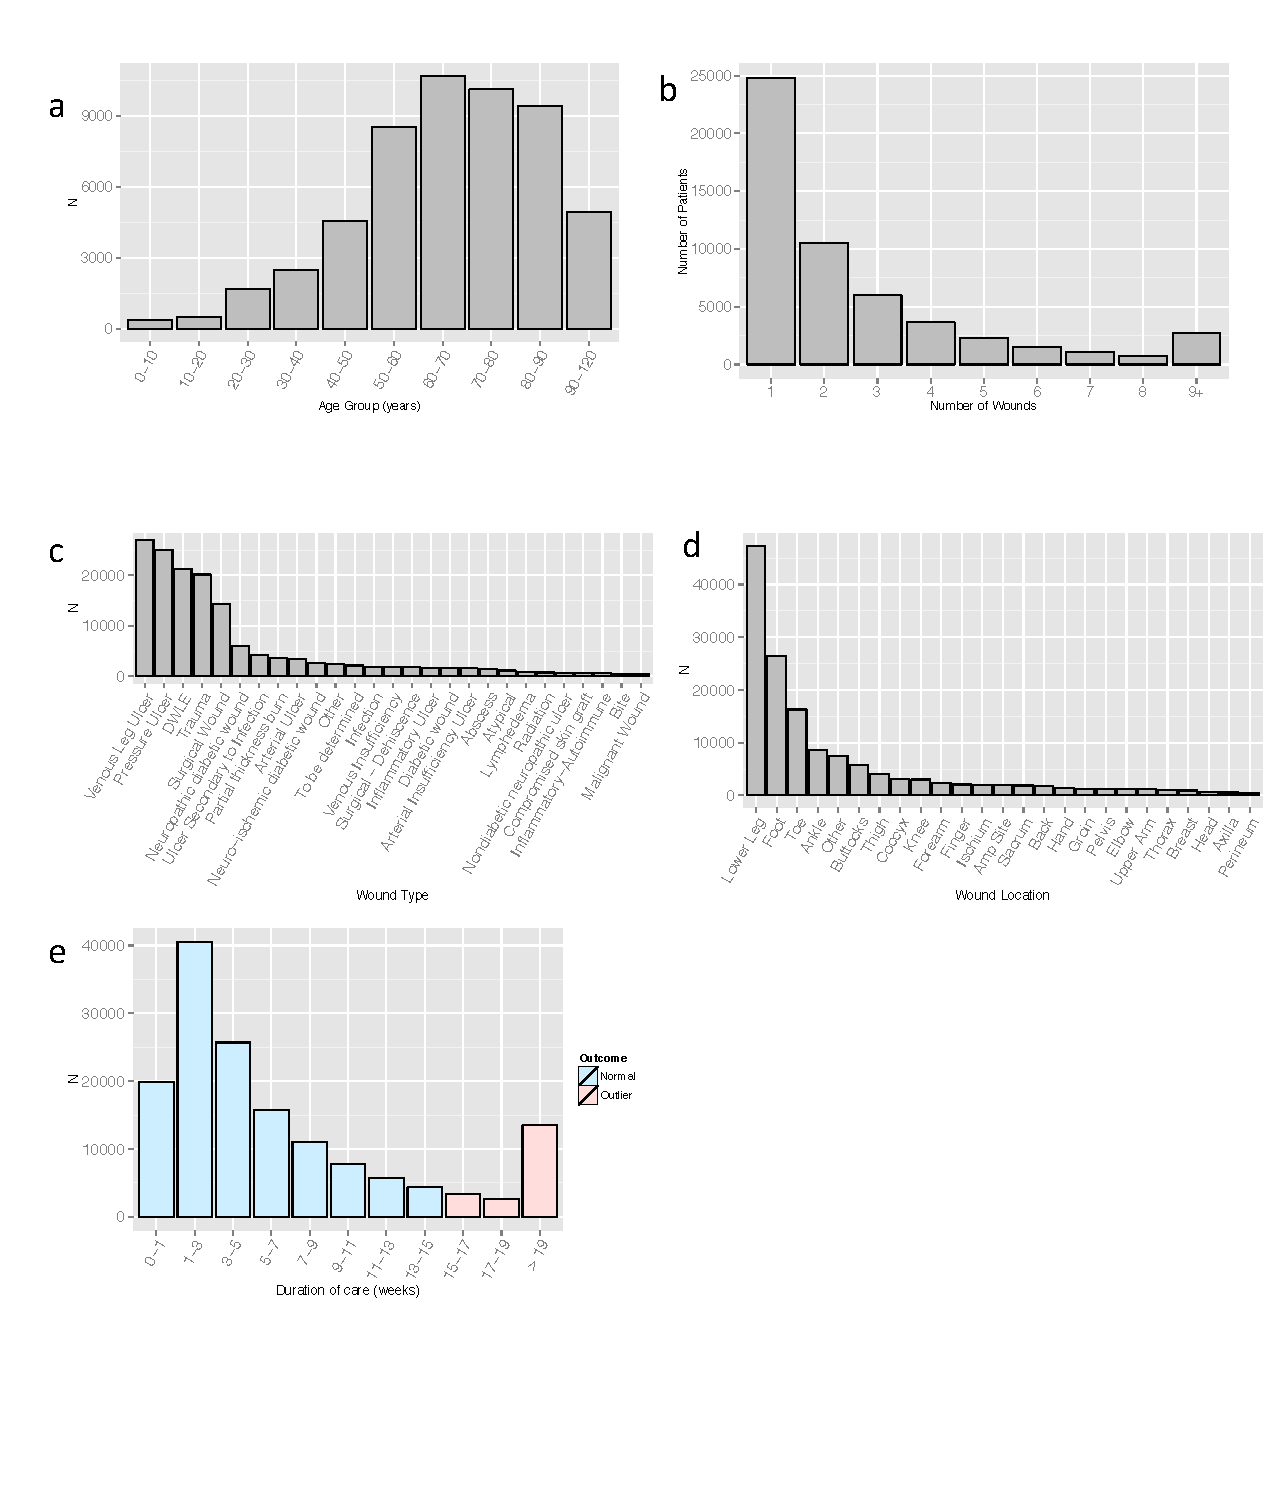
\includegraphics[width=0.9\linewidth]{ch5-figures/dataset_stats.pdf}
  \end{center}
  \caption[Wound healing dataset statistics]{Dataset statistics.}
  \label{fig:short}
\end{figure}

We removed any wounds that were unresolved by the end of the study
period unless the wound was already past the 15-week threshold for
delayed healing.  We also removed wounds with negative or very large
values for quantitative features (> 99.9th percentile) or with clearly
erroneous demographic information such as negative age.  This left us
with 150, 277 unique wounds for use in training and testing our
models.  The basic features for our models are the data for each wound
that is available at the time of the first wound assessment.

We performed additional pre-processing of the dataset as follows.
First, ICD9 codes were aggregated to 3 digit codes.  Second, wound
types and locations were aggregated into 40 and 37 values,
respectively, in order to account for variation between wound care
centers and misspellings.  Third, insurance information was aggregated
into four values - uninsured, private, Medicaid, and Medicare.

In this study, delayed wound healing is defined as taking 15 or more
weeks to heal; this threshold was chosen based on the advice of domain
experts from Healogics.  11.7\% of wounds meet this criterion in the
final dataset.

\subsection{Training and test splits}
We control the degree of non-stationarity seen by the models by
changing the way the dataset is split into training and test sets. A
naive strategy is to randomly assign wounds into the training and test
sets independently of each other, ignoring both time and the fact that
a single patient may have many wounds in the dataset.  This strategy
mirrors the assumption that the training and test data are from the
same distribution, and may be appropriate in settings in which this is
known or strongly suspected to be true.  A second strategy is to split
patients into training and test sets, and then assign wounds to
training and tests sets according to this patient assignment.  This
strategy respects the grouping of wounds by patient, but ignores time.
It approximates the population of patients undergoing a large change
in the future.  It may also yield a pessimistic estimate of model
performance because it is estimated on completely new patients; in
practice, a wound healing prediction model would see a mix of new and
previously seen patients.  Finally, we simulate a prospective setting
by assigning wounds from the end of the study period to the test set.
This procedure ignores the grouping of wounds by patient, but respects
the fact that we wish to make predictions about the future, and not
past events whose outcomes are unknown.  Under this setting, the model
development process “sees” the non-stationarity in the data.  In all
cases, data was split 4:1 into training and test sets.  In the case of
the simulated prospective setting, we performed this split by ordering
the wound assessments in time, and selecting the most recent fifth of
the data for the test set.  Figure 5.3 illustrates the split
strategies.

\begin{figure}
  \begin{center}
    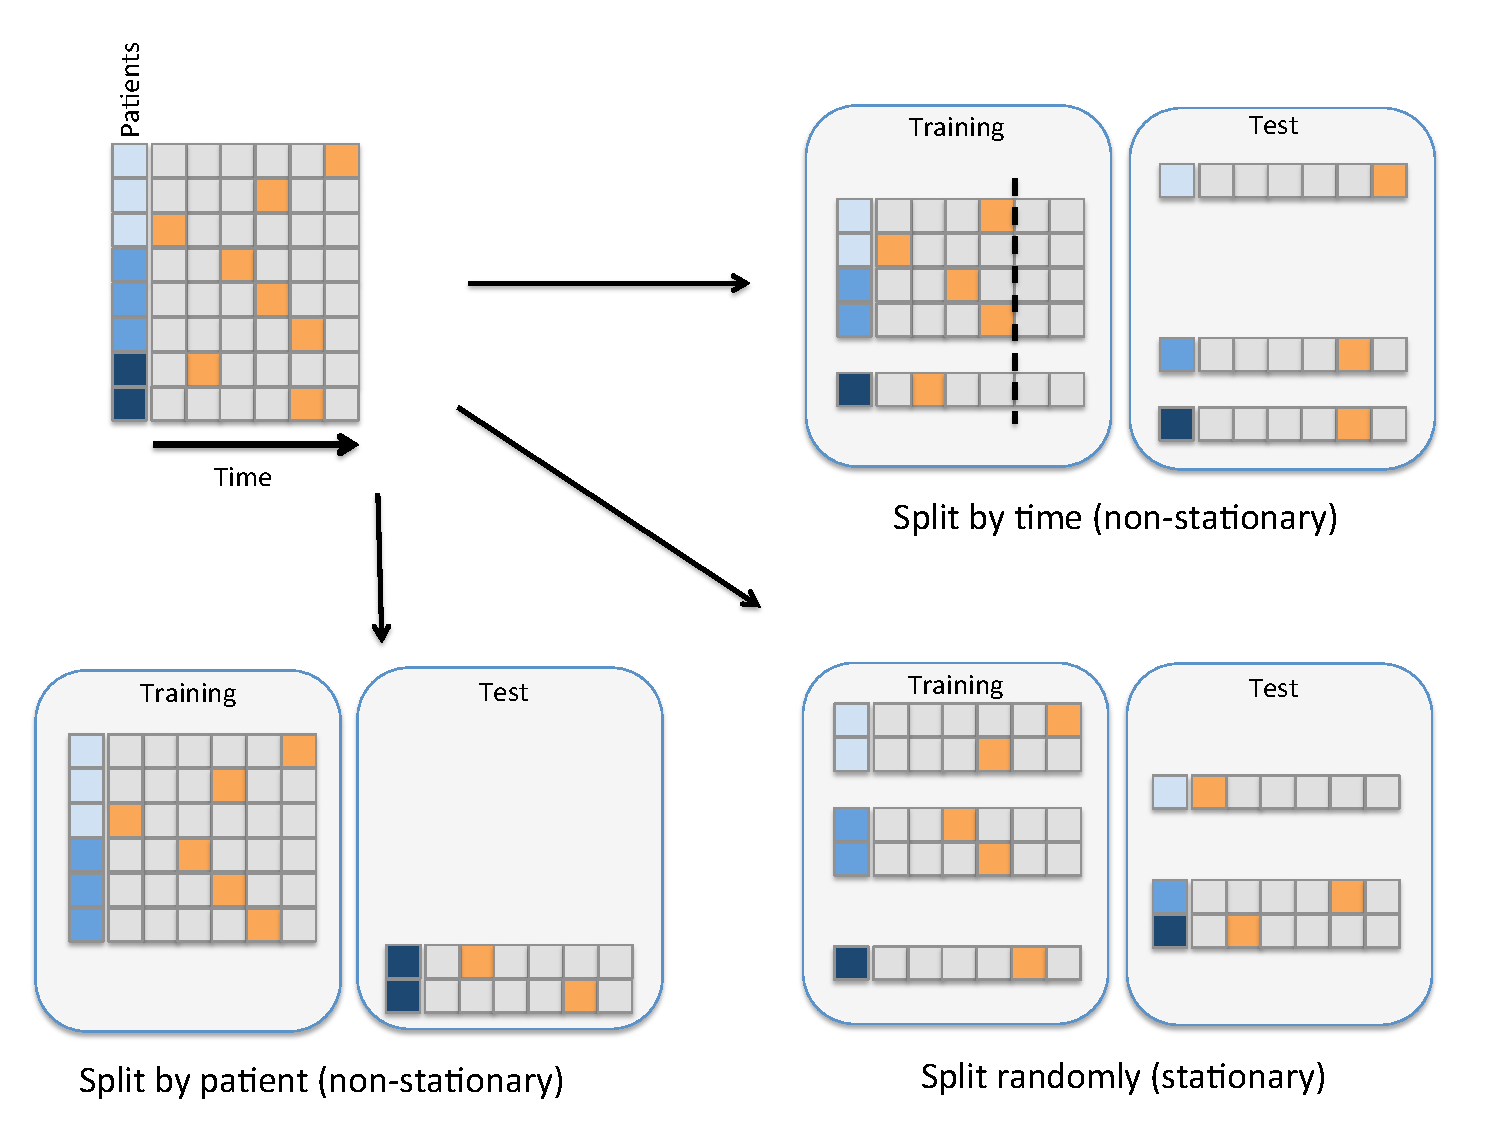
\includegraphics[width=0.9\linewidth]{ch5-figures/train_test_splits.pdf}
  \end{center}
  \caption[Approximating different degrees of stationarity using
    training and test splits] {Approximating different degrees of
    stationarity using training and test splits. Each row represents a
    wound.  The first column represents the patient for a given wound,
    and is color-coded such that different shades indicate different
    patients.  The time of the first wound assessment is indicated by
    the orange cell in the grey columns. In the random split, wounds
    are randomized into training and test directly. In the patient
    split, patients are randomized and wounds from a given patient go
    together. In the prospective split, we assign wounds from the end
    of the study period (shown by the dashed line) to the test set.}
  \label{fig:short}
\end{figure}


\subsection{Model choice}	
We evaluated the following models: L1 regularized linear regression
(LASSO) \cite{Lasso}, random forest (RF) \cite{Breiman2001,Liaw2002},
neural networks (NN) \cite{Goodfellow2013,Pylearn}, and gradient
boosted trees (GBM) \cite{Friedman2001,Ridgeway2007}. Each of these
models were fit to the training set for each of the splits, with their
respective hyperparameters tuned by cross validation on the training
data (LASSO) or on a held out subset of the training data.  Following
hyperparameter tuning, the models were refit to the entire training
set.

We also evaluated the use of two model ensemble methods – model
averaging and stacking – that combine the outputs of the above base
models \cite{Wolpert1992,Ting1999}.  Model averaging simply averages
the predictions of the base models.  We averaged the predictions of
the four base models trained on the full training sets.  In our
stacking experiments, we further split the training sets into two
parts – one for training base models, and another for training the
stacked model.  The stacked model was developed by fitting a GBM model
to the stacking dataset, which consisted of the original set of
features plus the posterior probabilities of the base models on the
stacking data.  

\subsection{Feature engineering}
We constructed additional features for each wound that measure the
change in quantitative variables such as wound dimensions between the
first and second assessments, and features that summarize the total
wound burden of each patient at the time of the first assessment, such
as number of wounds and total surface area. These features capture
intuition such as wounds that are decreasing in size during the first
week are more likely to heal well.  In all, a total of 833 features
were calculated for each wound, the bulk of which were binary
indicators for the levels of categorical variables (31 quantitative
versus 802 binary).

\subsection{Model evaluation}
A useful prognostic model for delayed wound healing should meet two
criteria.  First, it should be able to discriminate between positive
versus negative cases of the delayed wound healing.  Second, it should
output well-calibrated posterior probabilities of delayed wound
healing, i.e., the observed frequency of delayed wound healing should
be close to the predicted probability.  We evaluated the test set
performance of the various models under each all combinations of
training-test splits and feature sets.  Discriminative power on the
test data was evaluated using the Area under the ROC Curve (AUC),
which summarizes the sensitivity-specificity trade off across the
range of possible thresholds for calling an example a positive case.
We obtained 95\% confidence intervals for the AUCs by bootstrapping on
the test set.

Model calibration was evaluated by Brier reliability on the test data.
Brier reliability is a measure of calibration for probabilistic
predictions that are stratified into discrete groups, with lower
values indicating better agreement between the predictions in each
stratum and the observed frequency in those strata
\cite{Stephenson2008}.  It is equivalent to the mean squared deviation
between the predicted probability and the observed frequency within
each stratum, weighted by the number of observations in each stratum.
We formed strata by dividing the interval [0,1] into ten equal sized
bins.  In other words, all samples with predicted probabilities
between 0 and 0.1 fall into one bin, between 0.1 and 0.2 in the next,
etc.  We also evaluate calibration visually, by plotting reliability
diagrams: for each bin, the mean predicted probability is plotted
against the observed fraction of delayed wound healing
\cite{Degroot1982}.  Well-calibrated models will thus have its
reliability diagram near the diagonal line.

\section{Results}

\subsection{Discrimination}
Our measure of discriminative power is AUC in the test set (Figure
5.3), with 95\% confidence intervals obtained by bootstrapping for
10,000 iterations.  If the data generating process is stationary,
i.e., we split the dataset into training and test sets without using
patient and temporal information, we find that the non-linear models –
random forest, neural networks, and gradient boosted trees – have a
significant edge over the linear model (AUCs of 0.861, 0.854, and
0.861 versus 0.827 respectively).  Furthermore, combining the outputs
of these base models by model averaging and stacking provide
additional benefit over these non-linear models (AUCs of 0.872 and
0.876 respectively). These results suggest that one should use the
most complex model, the stacked GBM.

\begin{figure}
  \begin{center}
    \includegraphics[width=0.9\linewidth]{ch5-figures/discrimination.pdf}
  \end{center}
  \caption[AUC of models under different train-test splits]{AUC of
    models under different train-test splits. 95\% confidence
    intervals are shown.  The confidence intervals were obtained by
    bootstrapping on the test set.  }
  \label{fig:short}
\end{figure}

However, under the most realistic training/test split, i.e., a split
in which we trained on older data and evaluated on the most recent
data, we see that the relative performance of the models is almost the
same, with much less difference in performance between the base
models, and no benefit from model averaging and stacking (AUCs ranging
from 0.868 to 0.880 for the base models, and 0.881 for stacking).  We
note that the absolute performance is somewhat higher in the
prospective split setting, but do not generalize from this except to
note that it underscores the importance of non-stationarity.

When training and test data is split by patient, we find that gradient
boosted trees remain the best performing base model but with a smaller
advantage over the other models (AUC of 0.843 for gradient boosted
trees versus 0.819-0.826 for the other base models).  Model averaging
and stacking provide no additional benefit over gradient boosted trees
(AUC 0.846 for stacking versus 0.843 for gradient boosted trees).

We are also interested in the interaction between stationarity and the
use of domain specific features such as those that encode the initial
rate of wound closure.  Without using these features, we observe the
same trends described above, with gradient boosted trees being the
best performing base model under all training/test split procedures,
but with a smaller edge over the other models.  Table 5.1 summarizes
the discrimination performance.

\begin{table}
\begin{center}
  \begin{tabular}{|l|l|l|l|l|l|l||}
    \hline Model & \multicolumn{2}{|c|}{Random split} &
    \multicolumn{2}{|c|}{Prospective split} &
    \multicolumn{2}{|c|}{Patient split} \\
    \hline \hline
    & With & No & With & No & With & No \\
    & engineered & engineered & engineered & engineered & engineered & engineered \\
    & features & features & features & features & features & features \\
    \hline \hline
    Lasso &  0.827 & 0.807 & 0.868 & 0.851 & 0.819 & 0.791 \\
    RF & 0.861 & 0.837 & 0.870 & 0.843 & 0.825 & 0.788 \\
    NN & 0.854 & 0.835 & 0.87 & 0.846 & 0.826 & 0.807 \\
    GBM & 0.861 & 0.834 & 0.880 & 0.859 & 0.843 & 0.807 \\
    Mean & 0.872 & 0.850 & 0.881 & 0.858 & 0.840 & 0.809 \\
    Stacked & 0.876 & 0.875 & 0.881 & 0.860 & 0.841 & 0.808 \\
    \hline
\end{tabular}
\end{center}
\caption{Model discrimination measured by AUC.}
\end{table}

\subsection{Calibration}
Well-calibrated posterior probabilities are desirable for prognostic
models because they enable clinicians and patients to make decisions
that are informed by accurate estimates of the probabilities of the
outcomes of interest, which is especially important when performing
cost-benefit analysis of treatment options
\cite{Cook2007,Cook2008}. We evaluated model calibration by
calculating Brier reliability in the test set (Table 5.2). Here, the
general trend is that under all conditions, the linear and stacked
models are the best calibrated.  Figure 5.5 shows reliability diagrams
for the models under the various conditions.  In Figure 5.5a, we see
that under conditions of stationarity, we observe that the lasso,
neural net, and stacked models all have very good calibration, with
the mean posterior probability of delayed wound healing matching the
observed frequency of delayed healing in each of the bins.  The RF and
GBM models, on the other hand, seem to have relatively poor
calibration.  However, the situation changes under patient and
prospective splits.  Under conditions of non-stationarity, the GBM and
stacked models offer the best calibration.

\begin{figure}
  \begin{center}
    \includegraphics[width=0.9\linewidth]{ch5-figures/calibration.pdf}
  \end{center}
  \caption{Calibration of models under different train-test splits.}
  \label{fig:short}
\end{figure}


\begin{table}
\begin{center}
  \begin{tabular}{|l|l|l|l|l|l|l||}
    \hline Model & \multicolumn{2}{|c|}{Random split} &
    \multicolumn{2}{|c|}{Prospective split} &
    \multicolumn{2}{|c|}{Patient split} \\
    \hline \hline
    & With & No & With & No & With & No \\
    & engineered & engineered & engineered &
    engineered & engineered & engineered \\
    & features & features & features & features & features & features \\
    \hline \hline
    Lasso & 0.000299 & 0.000256 & 0.00146 & 0.00181 & 0.000372 & 0.000339 \\
    RF & 0.00205 & 0.0011 & 0.00347 & 0.00179 & 0.00163 & 0.00152 \\
    NN & 0.000151 & 0.000136 & 0.0021 & 0.000888 & 0.000194 & 0.000732 \\
    GBM & 0.00199 & 0.00227 & 0.000549 & 0.000702 & 0.000127 & 0.0000537 \\
    Mean & 0.00175 & 0.00161 & 0.00215 & 0.00147 & 0.000764 & 0.000602 \\
    Stacked & 0.0000793 & 0.000075 & 0.000401 & 0.000877 & 0.00035 & 0.000234 \\
    \hline
\end{tabular}
\end{center}
\caption[Model calibration measured by Brier calibration]{Model
  calibration measured by Brier calibration.}
\end{table}

\subsection{Model performance}
The goal of developing the model is to be able to predict delayed
wound healing on new wounds in the future.  Therefore, we view the
prospective split as providing the most relevant estimate of model
performance on unseen data.  We now focus on the performance of the
best performing model under the prospective split, gradient boosted
trees (GBM).  The GBM model achieved an AUC of 0.880 (95\% confidence
interval 0.872-0.885) over all wound types.  For the two wound types
previously examined by Margolis et al \cite{Margolis2003,Margolis2004}
(venous leg ulcers and diabetic neuropathic ulcers), we achieve AUCs
of 0.867 and 0.860 respectively, a significant improvement over the
previously reported best results of 0.71 and 0.70.  Performance in
other wound types well represented in the test set (N > 500) ranged
from 0.834 for trauma to 0.878 for pressure ulcers.  Table 5.3 shows
the AUC of this model on the test set by wound type for the ten wound
types most frequent in the test set.

\begin{table}
\begin{center}
\begin{tabular}{|c|c|c|c||}
\hline
&  & \multicolumn{2}{|c|}{AUC} \\
\hline
Wound Type & N & With & No \\
& & delta & delta \\
& & features & features \\
\hline \hline
Venous Leg Ulcer & 3646	& 0.867 & 0.853 \\
Pressure Ulcer & 2991 & 0.878 & 0.850 \\
Trauma & 2715& 0.864 & 0.834 \\
Neuropathic diabetic wound & 2596 & 0.860 & 0.833 \\
Surgical Wound & 1791 & 0.862  & 0.850 \\
Neuro-ischemic diabetic wound & 1180 & 0.874 & 0.838\\
Diabetic wound, lower extremity & 988 & 0.846 & 0.815\\
Abscess & 659 & 0.843 & 0.790 \\
Arterial Insufficiency Ulcer & 593& 0.856 & 0.843 \\
Infection & 381 & 0.826 & 0.806 \\
\hline
\end{tabular}
\end{center}
\caption[Performance of GBM by wound type, prospective
  split]{Performance of the GBM model by wound type under the
  prospective train-test split.  We show results for the ten most
  prevalent wound types in the test set.}
\end{table}

\section{Discussion}
\subsection{A predictive model of delayed wound healing}
We developed a prognostic model for delayed wound healing outcomes
that uses data routinely captured in EHRs during the first two weeks
of care at wound centers.  The model achieves best-to-date
discriminative power and calibration on validation data.  Unlike
previous work, our model is also applicable to the full range of wound
types.  Furthermore, by changing the cutoff threshold, it is possible
to make trade offs between positive predictive value and sensitivity
(recall) for specific uses of the model (Figure 3b).  For instance, it
may be desirable to trade off low positive predictive value for a high
sensitivity when making decisions regarding referral to specialized
wound care centers.  Once referred to a wound center, however, it may
be desirable to have a high positive predictive value and sacrifice
sensitivity when making decisions about high cost interventions that
may improve outcomes in potentially problematic cases.  Because the
model outputs are well-calibrated probabilities, they can be used
directly to make informed referral or intervention decisions that
helps care providers and patients.

Our approach does have limitations. Although our model was developed
on data from 68 geographically distributed wound care centers in 26
states, it may not generalize to centers other than those that
participated in this study.  Indeed, we observe considerable
inter-center variability in practices and patient populations.
Second, it is possible that the model may not generalize to cases
outside wound care centers, limiting its utility for making referral
decisions.  Third, in contrast with previous work, we have traded
simplicity for accuracy.  The simple models by Margolis et al. can be
applied by basic arithmetic.  In exchange, however, we have achieved
significantly higher accuracy.  We would argue that in the age of
widespread and growing adoption of EHRs, it is time to shift some of
the burden of such prognostication to automated systems.

These limitations notwithstanding, our model, to the best of our
knowledge, is the first that has been developed and validated on the
full diversity of patients and wound types seen in clinical practice.
It achieves significantly better discrimination than those of previous
efforts, and is a case study for the meaningful secondary use of
routinely collected EHR data to improve treatment strategies.

\subsection{Non-stationarity in predictive modeling}
The increasing abundance of EHR derived clinical data enables
researchers to apply increasingly sophisticated models to clinical
problems.  However, we argue that the real world processes generating
this data are highly non-stationary, driven by factors such as rapidly
evolving financial incentives, clinical practice, and adoption of and
adaptation to new technology.  We have investigated what these changes
imply for researchers in biomedical informatics, especially those
engaged in predictive modeling.

We have presented a case study in which a large dataset was used to
predict delayed wound healing in outpatient wound care centers.  By
changing the way in which we split the dataset into training and test
sets we were able to evaluate the impact of non-stationarity on the
models.  We found that under a stable data distribution, there was
substantial benefit from complex models, including ensemble methods
such as model averaging and stacking, over a baseline of a regularized
linear classifier.  However, this benefit was greatly diminished when
we trained the models on older data and evaluated them on the most
recent data.  We argue that this “prospective evaluation” scenario
provides the most relevant evaluation of model performance.  Our
experience in this study suggests the following lessons.

First, when one is uncertain about the possibility or presence of
non-stationarity, it may be best to stick with simpler models.
Conversely, when one is confident that the data distribution is stable
and will remain so for some time, then more complex models, including
ensemble methods such as model averaging and stacking, may provide
substantial benefits with respect to discriminative power and
calibration.  Second, given the choice between spending resources on
increasingly sophisticated models and the engineering of
domain-specific features, it may be advisable to focus on the latter.
In this dataset, the benefit from using features that encode the
initial rate of wound closure are substantial, and consistent across
all conditions, implying that the utility of these features is stable
even when the data distribution is non-stationary.  Of course it is
possible that particular features may not be so robust in other
prediction problems.

Finally, we argue that the most important lesson to draw from this
study is that one ought to be very clear about the intended purpose of
the model being developed, and use a model development process that
reflects that purpose.  For instance, if one is developing a model
whose purpose is cohort selection, e.g., a classifier for finding
patients with a specific condition, then making predictions on unknown
cases from the past is a useful goal, and it may make sense to train
and evaluate models without regard to time.  In the case of our wound
healing prediction model, however, it does no good to evaluate by
predicting delayed wound healing on past cases.  Rather, we are
interested in making predictions on new cases in the future, on a mix
of previously seen and completely new patients.



